% \begin{tikzpicture}[scale=1.5]

%     % 绘制坐标轴
%     \draw[->] (-0.5,0) -- (2.5,0) node[right] {$\Re$};
%     \draw[->] (0,-1.5) -- (0,2.5) node[above] {$\Im$};
    
%     % 定义积分路径的控制点
%     \coordinate (A) at (0.4,0.8);
%     \coordinate (B) at (1.5,1.2);
%     \coordinate (C) at (2,0.5);
%     \coordinate (D) at (1.2,-0.5);
    
%     % 绘制复平面上的积分路径
%     % \draw[thick, red] (0,0) -- (A) .. controls (B) .. (C) -- (D) -- (0,0);
%     % \draw[thick, red] (0,0) -- (A) .. controls (B) .. (C) -- (D) .. (0,0);
    
%     % 贝叶斯曲线参数
%     \def\a{-0.5}
%     \def\b{-1}
%     \def\c{0}
%     \def\d{0.5}
%     % 绘制贝叶斯曲线
%     % \draw[thick, blue] plot[domain=-1:2, samples=100] (\x, {\a + \b * exp(-(\x - \c)^2 / (2 * \d^2))});

%     \draw[thick, blue] plot[domain=0.5:2, samples=100] (\x, {\a + \b * \x + \c * \x^2 + \d * \x^3});

%     % 绘制复平面上的积分路径标记
%     % \node[black, above right] at (A) {$z_1$};
%     % \node[black, above] at (B) {$z_2$};
%     % \node[black, above right] at (C) {$z_3$};
%     % \node[black, below right] at (D) {$z_4$};
    
%     % 绘制复平面上的积分起点和终点
%     \filldraw[black] (0,0) circle (0.03) node[below left] {$O$};
%     \filldraw[black] (1.2,-0.5) circle (0.03) node[below right] {$z$};
    
%     % 绘制复平面上的积分路径标记
%     % \draw (0.8,1) node {$\Gamma$};
    
%     \end{tikzpicture}








\tikzset{every picture/.style={line width=0.75pt}} %set default line width to 0.75pt        

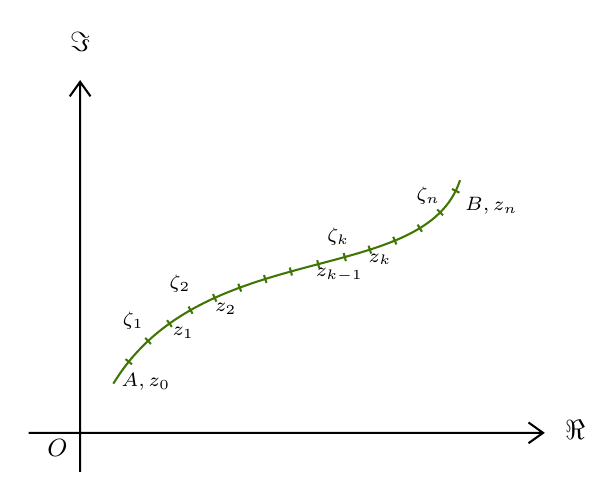
\begin{tikzpicture}[x=0.75pt,y=0.75pt,yscale=-1,xscale=1]
%uncomment if require: \path (0,300); %set diagram left start at 0, and has height of 300

%Shape: Axis 2D [id:dp2198947180733517] 
\draw  (83,214.11) -- (330.8,214.11)(107.78,45) -- (107.78,232.9) (323.8,209.11) -- (330.8,214.11) -- (323.8,219.11) (102.78,52) -- (107.78,45) -- (112.78,52)  ;
%Curve Lines [id:da014028466733404077] 
\draw [color={rgb, 255:red, 65; green, 117; blue, 5 }  ,draw opacity=1 ]   (123.8,190.4) .. controls (123.44,190.89) and (125,188.45) .. (125.62,187.51) .. controls (169.74,120.08) and (274.04,143.68) .. (290.8,92.4)(129.64,178.59) -- (132.75,181.1)(139.15,168.38) -- (141.88,171.31)(149.65,159.83) -- (151.98,163.08)(159.97,153.25) -- (161.95,156.73)(171.78,147.26) -- (173.43,150.9)(183.98,142.28) -- (185.36,146.03)(196.37,138.08) -- (197.56,141.9)(208.77,134.45) -- (209.84,138.3)(221.98,130.9) -- (223,134.77)(234.73,127.48) -- (235.79,131.34)(246.75,123.93) -- (247.97,127.74)(258.61,119.66) -- (260.14,123.35)(270.38,113.8) -- (272.46,117.22)(279.82,106.5) -- (282.65,109.33)(286.93,96.63) -- (290.52,98.4) ;

% Text Node
\draw (90.5,215.9) node [anchor=north west][inner sep=0.75pt]  [font=\small]  {$O$};
% Text Node
\draw (340,206.4) node [anchor=north west][inner sep=0.75pt]    {$\Re $};
% Text Node
\draw (101.5,19.4) node [anchor=north west][inner sep=0.75pt]    {$\Im $};
% Text Node
\draw (126.3,183.8) node [anchor=north west][inner sep=0.75pt]  [font=\scriptsize]  {$A,z_{0}$};
% Text Node
\draw (245.3,126.3) node [anchor=north west][inner sep=0.75pt]  [font=\scriptsize]  {$z_{k}$};
% Text Node
\draw (219.8,133.3) node [anchor=north west][inner sep=0.75pt]  [font=\scriptsize]  {$z_{k-1}$};
% Text Node
\draw (171.3,150.3) node [anchor=north west][inner sep=0.75pt]  [font=\scriptsize]  {$z_{2}$};
% Text Node
\draw (126.8,154.3) node [anchor=north west][inner sep=0.75pt]  [font=\scriptsize]  {$\zeta _{1}$};
% Text Node
\draw (150.8,161.8) node [anchor=north west][inner sep=0.75pt]  [font=\scriptsize]  {$z_{1}$};
% Text Node
\draw (291.8,99.3) node [anchor=north west][inner sep=0.75pt]  [font=\scriptsize]  {$B,z_{n}$};
% Text Node
\draw (149.3,136.8) node [anchor=north west][inner sep=0.75pt]  [font=\scriptsize]  {$\zeta _{2}$};
% Text Node
\draw (225.3,113.8) node [anchor=north west][inner sep=0.75pt]  [font=\scriptsize]  {$\zeta _{k}$};
% Text Node
\draw (268.3,94.3) node [anchor=north west][inner sep=0.75pt]  [font=\scriptsize]  {$\zeta _{n}$};


\end{tikzpicture}

